\documentclass[oneside]{article}
\usepackage{graphicx} % Required for including images
\usepackage[paper=A4,pagesize]{typearea}
% \usepackage{subfig} % Required for creating figures with multiple parts (subfigures)
\usepackage{soul}
\usepackage{setspace}
\usepackage{floatrow}
\floatsetup[table]{capposition=top}
\usepackage{amsmath,amssymb,amsthm} % For including math equations, theorems, symbols, etc
\usepackage{csquotes}
\usepackage{mathrsfs}
\usepackage{bm}
\usepackage{fancyhdr}
\usepackage{epstopdf}
\usepackage{subcaption}
\usepackage{listings}
\usepackage[dvipsnames]{xcolor}
\definecolor{Light}{gray}{.90}
\lstset{basicstyle=\ttfamily\footnotesize,
  showstringspaces=false,
  commentstyle=\color{red},
  keywordstyle=\color{blue},
  backgroundcolor=\color{Light},
}
%for adding notes
\usepackage[many]{tcolorbox}
\newtcolorbox{story}[1][]{
  width=\textwidth,
  fonttitle=\bfseries,
  breakable,
  fonttitle=\bfseries\color{Brown},
  colframe=SeaGreen,
  colback=SeaGreen!10
  #1}
\newcommand\StoryNote[3][]{%
  \marginnote[#1]{%
    \makebox[0pt][l]{\begin{mynote}[label=#3]
    #2
    \end{mynote}}}%
}
\usepackage{polynom}
\usepackage{floatrow}
\usepackage{multirow}
\usepackage[british]{babel} %for hyphenations etc.
\usepackage{pdflscape}
\usepackage{ifthen}
\usepackage{color}
\usepackage{tikz}
\usetikzlibrary{matrix,arrows.meta,quotes,shadows,decorations.pathreplacing,positioning,fadings}
\usepackage{cfr-lm} %imported for neural net drawing
% import this so we use the nice TeX font
\usepackage{lmodern}
\usepackage{hyperref}
\hypersetup{
    colorlinks=true,
    linkcolor=blue,
    citecolor=blue,
    filecolor=magenta,      
    urlcolor=blue,
  }
\hypersetup{linktocpage} %so TOC only links the page numbers
\usepackage{nomencl}
\makenomenclature
%% Grouping for Nomenclature
\usepackage{etoolbox}
\renewcommand\nomgroup[1]{%
  \item[\bfseries
  \ifstrequal{#1}{A}{Abbreviations}{%
  \ifstrequal{#1}{S}{Symbols}{}}%
]}
% Table float box with bottom caption, box width adjusted to content
\newfloatcommand{capbtabbox}{table}[][\FBwidth]
\usepackage{blindtext}
\usepackage{array}
% 
%MY NEW COMMANDS
\newcommand{\mb}[1]{\mathbf{#1}}
\newcommand{\N}{\mathcal{N}}
\newcommand{\E}{\mathbb{E}}
% Table alignment
\newcolumntype{L}[1]{>{\raggedright\let\newline\\\arraybackslash\hspace{0pt}}m{#1}}
\newcolumntype{C}[1]{>{\centering\let\newline\\\arraybackslash\hspace{0pt}}m{#1}}
\newcolumntype{R}[1]{>{\raggedleft\let\newline\\\arraybackslash\hspace{0pt}}m{#1}}
%
%
% Section referencing
\newcommand{\sref}[1]{\S\ref{#1}}
\sethlcolor{Light}
\newcommand{\hltexttt}[1]{\texttt{\hl{#1}}}
% 
%
%Document specific settings
\linespread{1.5}
%macro so when \textcite or \citeauthor is used, the et al. will appear in italicsc
%
\usepackage[style=ieee, backend=biber,
mincitenames=1,maxcitenames=2,
isbn=false, doi=false, url=false]{biblatex}
\addbibresource{ref.bib}
\DefineBibliographyStrings{english}{%
    andothers = {\em et\addabbrvspace al\adddot}
  }

\renewbibmacro{in:}{}
\AtEveryBibitem{%
  \clearlist{language}%
}
%
% 
%
\fancypagestyle{main}{
\fancyhead{}
\fancyfoot{}
\fancyhead[L]{\ifthenelse{\isodd{\value{page}}}{\leftmark}{\thepage}}
\fancyhead[R]{\ifthenelse{\isodd{\value{page}}}{\thepage}{}}
}
%so footnotes don't run over to next pages
\interfootnotelinepenalty=10000
%
%
\fancypagestyle{nomenclature}{
\fancyhead{}
\fancyfoot{}
\fancyhead[L]{\ifthenelse{\isodd{\value{page}}}{NOMENCLATURE}{\thepage}}
\fancyhead[R]{\ifthenelse{\isodd{\value{page}}}{\thepage}{}}
}
%
\begin{document} 
%
%Set the page style to main
\pagestyle{main}
%
%
%
\title{A BRAG Guide to HPC}
\date{}
\author{Ethan Goan}
\maketitle
\begin{figure}[!h]
  \centering
  
\includegraphics[scale=0.5]{./figs/qut.eps}
\end{figure}
\begin{center}
  Version 0.1 - Last Updated 20/07/2018
\end{center}
\tableofcontents
%
\newpage
%
\section*{Preface}
\addcontentsline{toc}{section}{Preface}
As the size of data sets increase and models become increasingly complex, the need for High Performance Computing (HPC) systems becomes increasingly prominent. The purpose of this document is to provide a gentle introduction to using the High Performance Computing (HPC) cluster from a statistical perspective. Sample scripts and examples are provided, and intended to serve as a basis for any future work people may need. From these examples provided in this guide, you will be able to modify them to your need to make submitting jobs to HPC as easy as possible. It is hoped that this document can serve as a reference guide, a first port of call to those who might not be familiar with HPC and want to benefit from the facilities. It is also important to note that the scheduler used at QUT is used extensively at many universities and research facilities, so knowledge of QUT's HPC system will extend much past QUT.
%
%
\par
%
%
This guide will start with a brief introduction to UNIX like systems, and how to navigate a command line. The guide will also show how you can bypass much of the command line use, to remove as much prerequisite knowledge of UNIX as possible. The HPC scheduler is then introduced, along with modules currently installed on the cluster and how to access them. Sample scripts are provided with instructions on how to submit both batch and interactive jobs. Instructions on how to customise your personal environment and install your own packages is also provided. This guide will primarily focus on programs written in R, though instructions can be followed with only slight modifications for other platforms and languages such as MATLAB, Python and Mathematica.
%
%
\par
%
%
Additional tips and tricks to help get the most out of the cluster are also provided. The tips include suggestions on how to (hopefully) simplify your HPC experience. This will be demonstrated through sample scripts that you can run yourself.
%
%
\par
%
%
From my experience, others have often already encountered and solved many of the problems. I have also noticed that more often than not, others with more experience have developed far more elegant solutions to the same problems I have faced. It is for this reason that I have decided to make this document, to impart some of the knowledge that others with considerably more experience have passed on to me. In this spirit, I am happy for this to be a living document that all can edit, to provide your own tips and tricks to solve potential problems you think others might encounter. Through collaboration, we can all benefit from each others work and streamline our development process, by not needlessly addressing a problem others have already solved.
%
%
%
%
%
\newpage
\section{Introduction and Preliminaries}
%
%
%
%
The QUT HPC facilities provide access to,
\begin{itemize}
\item 212 compute nodes
\item 3780 Intel Xeon Cores
\item Approx. 200G B RAM per Compute Nodes
\item 34 TB of main storage
\item 1800 TB additional storage in file store
\item 24 Tesla GPUs
\item Visualisations services and more
\end{itemize}
%
%
%
\subsection{Getting HPC Access}
Before accessing HPC, you will first need to apply for access. This can be done via HiQ by following the instructions on this link \href{https://qutvirtual4.qut.edu.au/group/research-students/doing-your-research/specialty-research-facilities/apply-for-a-hpc-account}{here}. Access will usually be granted in a couple of days at the most.
%
%
\par
%
%
Once access has been granted, you will need a program to access HPC. If you are using a Linux or Mac, you won't need to install anything, though if you are using Windows, it is recommended to use the program PuTTY \cite{putty}. Instructions on logging in to HPC for each OS are given here.
%
%
\subsubsection{Mac and Linux}
To log into HPC, we will be using the Secure SHell (SSH) protocol, which we can access through the command line on Mac and Linux devices. To login, first open a command line prompt (terminal) in your computer. To login, you will need to type in,
\\
\par
\begin{minted}[bgcolor=Light, frame=single, fontsize=\footnotesize, fontfamily=courier]{bash}
  ssh <your_qut_id>@lyra.qut.edu.au
\end{minted}
\\
where you will replace \hltexttt{<your\_qut\_id>} with your QUT username, ie.
\\
\par
\begin{minted}[bgcolor=Light, frame=single, fontsize=\footnotesize, fontfamily=courier]{bash}
  #if you applied for HPC access with staff account
  ssh jane.doe@lyra.qut.edu.au
  #if you applied for HPC access with student account
  ssh n12345678@lyra.qut.edu.au
\end{minted}
%
%
%
%
\subsubsection{Windows}
To login on windows, first install PuTTY by following the instructions \href{https://www.putty.org/}{here}. Once downloaded, open the putty window and enter \hltexttt{lyra.qut.edu.au} into the bar as shown in Figure \ref{fig:putty}. You will then have to enter your QUT username and password.
\begin{figure}[!h]
  \centering
  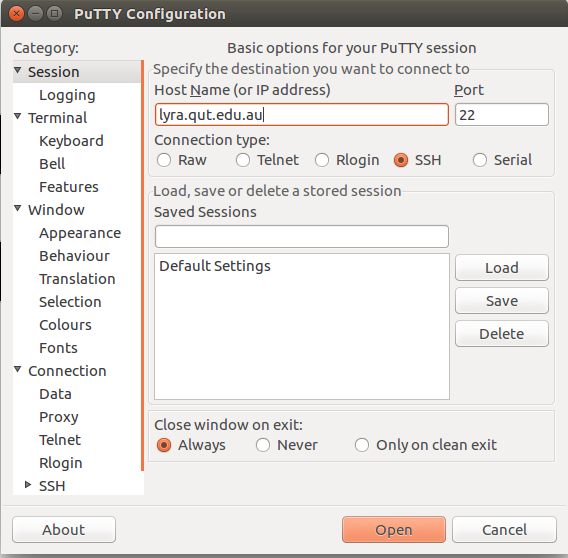
\includegraphics[width=0.5\linewidth]{./figs/putty.png}
  \caption{Example PuTTY window}
  \label{fig:putty}
\end{figure}
%
%
\subsection{Once Logged In}
After following the previous commands you will be logged into the head node of the Lyra HPC cluster. Though you will now be logged in, you have not been allocated any computational resources yet. The head node is available to all users once logged in, and is designed for performing only simple tasks, such as text editing or checking on currently running jobs. If you do start running a program that is computationally expensive, the HPC staff may intervene and kill your process. Running programs from the head node also has the potential to crash the HPC infrastructure. Section \ref{sec:submitting} will explain how to begin submitting jobs using resources you have requested.
%
%
\par
%
%
\subsection{Transferring Files to HPC}
Now that you have access to HPC, you will want to transfer some code over so you can start running some jobs. There are a few ways to do this, though this guide will cover the easier/most prominent ways to do this.
%
%
\par
%
%
To get your code onto HPC, I would recommend using Git and cloning your repo onto HPC. If you are unsure on how to use Git, I would strongly recommend you take some time to learn some basics and start using it for your software projects. Knowledge of Git is not required for this guide, but it will make your software development life significantly better, and allow you to distribute your research much easier.
%
%
\par
%
%
You can clone your repo to HPC via the terminal that is connected to HPC by running the command,
\\
\par
\begin{minted}[bgcolor=Light, frame=single, fontsize=\footnotesize, fontfamily=courier]{bash}
  #change to the home directory
  git clone <remote_url_for_your_repo>
\end{minted}
%
%
\subsection{Mounting HPC Drive on Your Machine}
Directions for how to mount your HPC home drive onto your desktop machine can be found on the \href{https://wiki.qut.edu.au/pages/viewpage.action?pageId=244125273}{QUT HPC Wiki}. The QUT HPC Wiki can be a reasonable source for information, though many of the guides are incomplete, or hard to follow for a new user (hence the creation of this guide!), though the methods for mounting a drive are good. I will provide some alternative methods for mounting a drive here, so feel free to follow either one.
%%
%
%
\subsubsection{Mac and Linux}
It is also helpful to be able to transfer other files to and from HPC. The easiest way to do this is to mount a network directory, so you can copy and paste files to and from HPC just like you would on your desktop/laptop. Instructions on how to do this for Windows, Mac and Linux using SSHFS is provided \href{https://www.digitalocean.com/community/tutorials/how-to-use-sshfs-to-mount-remote-file-systems-over-ssh}{here}. After you install the required programs, you can mount the directory by creating a folder on your desktop where you want to mount your HPC files by running the following command into a terminal that is not logged on to HPC,
%
%
\\
\par
\begin{minted}[bgcolor=Light, frame=single, fontsize=\footnotesize, fontfamily=courier]{bash}
  #run these commands on YOUR MACHINE
  #ie in a new terminal that is not logged on to HPC
  #create a directory on your machine where we will mount the
  #HPC network drive
  mkdir ~/lyra #new folder will be in home directory
  #now mount your HPC home drive to this lyra folder
  #all of this in a single line/command
  sshfs <your_qut_username>@lyra.qut.edu.au:/home/<your_qut_username> ~/lyra
\end{minted}
% 
%
%
\par
\begin{story}
  \textbf{NOTE:}
  \\
  The rest of the commands shown throughout this guide should be run in a terminal that is logged in to HPC
\end{story}
% 
%
\subsubsection{Windows}
For Windows machines, called \href{https://www.nsoftware.com/netdrive/sftp/}{SFTP Net Drive} will allow you to mount your home drive on HPC to your laptop/desktop. After you install the program, type in \hltexttt{lyra.qut.edu.au} as the server, and enter your QUT username and password. This will mount your HPC home drive to your machine in a new drive that can be found in My Computer on your machine.
%
\par
%
An alternative program called \href{https://winscp.net/eng/download.php}{WinSCP} will do allow you transfer files to and from HPC. This is (slightly) less nice to use, but the option is there if you like.
%
%
\subsection{Logging in When Not On QUT's Network}
%
%
Up until now, you would have been required to be at QUT and directly connected to the network to log in to HPC. We can access HPC from off campus by using the \href{https://secure.qut.edu.au/ithelpdesk/qut/softwaredownloads/downloads.jsp}{Cisco Remote Access Client} to open a VPN connection to QUT's network. To open the VPN connection, install the remote client from \ref{https://secure.qut.edu.au/ithelpdesk/qut/softwaredownloads/downloads.jsp}{here}. For the VPN address, use \texttt{sas.qut.edu.au}, then use your QUT staff or student credentials to login. After you have opened the VPN connection, you can log in to HPC using the exact same instructions used previously. This means you can now access HPC from home, from the Botanic Gardens, overseas, or practically anywhere you have an internet connection!
%
%
\par
\begin{story}
  \textbf{NOTE:}
  \\
  You won't be able to open a VPN connection on some networks, such as Eduroam.
\end{story}

%%% Local Variables:
%%% mode: latex
%%% TeX-master: "main"
%%% End:
%
%
\section{Submitting Jobs}
\label{ref:submitting}
%
%
%
Whilst it may seem like ample resources are available, they are finite and accessed by many people, thus access to these services needs to be managed. Access to computing resources is scheduled by the Portable Batch System (PBS). Before you run any software, you must tell the PBS manager what resources you require and how long you will need them for. This is done by submitting jobs.
%
%
\par
%
%
There are two main types of jobs you can submit to HPC; interactive and batch jobs. Interactive jobs provide you with an active terminal similar to what you will currently use on your desktop. Interactive jobs are useful for debugging and ensuring all of your code can run.
%
%
\par
%
%
Interactive jobs are often convenient, though you need to have your interactive session open for the job to continue. Batch jobs are intended for jobs that will need to run for longer, or when multiple jobs need to be submitted. Unlike interactive jobs, after you submit a batch job, you can close your connection to HPC altogether, go get a coffee, put your feet up and relax while your job processes on HPC in the background.
%
%
%
\par
We will first start with interactive jobs, and then show how we can move our work to batch jobs later on.
%
%
%
\subsection{Interactive Jobs}
To submit a job to HPC, we use the \hltexttt{qsub} command, along with a few arguments to tell the scheduler what resources we require, and how long we need them for. To submit an interactive job, run the following command,
%
%
\\
\par
\begin{minted}[bgcolor=Light, frame=single, fontsize=\footnotesize, fontfamily=courier]{bash}
  #submit an interactive job to HPC
  #replace the HH:MM:SS with the amount of time you
  #expect your job to run
  #Replace XXX with the amount of RAM you need
  #Replace YYY with the number of CPUS you need
  #Replace ZZZ with the name of your job
  #you can call it whatever you like :)
  qsub -I -S /bin/bash -l walltime=HH:MM:SS,mem=XXXg,ncpus=YYY -N ZZZ
\end{minted}
%
\\
%
Change the variables supplied here with the time and resources required for your work. After running this command, you will have to wait for your requested resources to be allocated to you. The time taken for your job to be accepted will depend on the amount of resources you requested. If you asked for 8 GB of RAM, 2 CPUs for only a couple hours, your job should be accepted within a minute or so. If you request 100 GB, 20 CPUs for 12 days, expect to wait a very long time for your interactive job to be accepted.\footnote{You can request these resources, but will need to submit a batch job. See section \ref{sec:batch} for instructions on how to submit these.}

\subsection{Modules}
Now that you have transferred your code across over to HPC and have been allocated resources for a job, you can start loading and installing the required packages you need. HPC has many programs already installed, though they aren't initially loaded when you log in. These pre-installed programs are stored as \textit{modules} that need to be first loaded before you can use them. To see the modules currently installed on HPC, run the command,
%
%
\\
\par
\begin{minted}[bgcolor=Light, frame=single, fontsize=\footnotesize, fontfamily=courier]{bash}
  #see what modules are available
  module avail
\end{minted}
From the output of this, you may begin to appreciate why not all of the packages are loaded on startup, there is an awful lot of them. You can search through the output to find any modules you are interested in. Once you have found the module you are interested in, you can load it with the \hltexttt{module load} command. An example of common modules that might be helpful are listed here.
%
\\
%
\subsubsection{R Modules}
Output of \hltexttt{module avail r}
\begin{minted}[bgcolor=Light, frame=single, fontsize=\footnotesize, fontfamily=courier]{bash}
  #load in R (output of module avail r)
  -------------- /pkg/suse12/modules/lang --------------
  r/3.1.0-foss-2016a              r/3.4.2-foss-2017a             
  r/3.2.0-foss-2015a-bare         r/3.5.1-foss-2018a             
  r/3.3.1-foss-2016a              r/3.6.1-foss-2019a             
  r/3.3.1-intel-2016b(default)    r/3.6.2-foss-2019b
  r/3.4.2-bioconductor-foss-2017a r/4.0.3-foss-2020b
\end{minted}
%
%
\subsubsection{Matlab Modules}
Output of \hltexttt{module avail matlab}
\begin{minted}[bgcolor=Light, frame=single, fontsize=\footnotesize, fontfamily=courier]{bash}
  -------------- /pkg/suse12/modules/math --------------
  matlab/2016b matlab/2017a matlab/2017b
  matlab/2018b matlab/2019a matlab/2021a
\end{minted}
%
%
\subsubsection{Mathematica Modules}
Output of \hltexttt{module avail mathematica}
  \begin{minted}[bgcolor=Light, frame=single, fontsize=\footnotesize, fontfamily=courier]{bash}
  -------------- /pkg/suse12/modules/math --------------
  module load mathematica/11.2.0-linux-x86_64
\end{minted}

\subsubsection{Python Modules}
Output of \hltexttt{module avail python}
\begin{minted}[bgcolor=Light, frame=single, fontsize=\footnotesize, fontfamily=courier]{bash}
  -------------- /pkg/suse12/modules/lang --------------
python/2.7.10-intel-2015b                  python/2.7.15-intel-2018b
python/2.7.11-foss-2016a                   python/2.7.16-foss-2019a
python/2.7.11-intel-2016a                  python/2.7.16-gcccore-7.3.0
python/2.7.11-intel-2016b                  python/2.7.16-gcccore-8.3.0
python/2.7.11-iomkl-2016.07                python/2.7.18-gcccore-10.2.0
python/2.7.11-iomkl-2016.09-gcc-4.9.3-2.25 python/2.7.18-gcccore-9.3.0
python/2.7.12-foss-2016a-repair            python/2.7.5-foss-2017a
python/2.7.12-foss-2016b                   python/3.5.1-foss-2016a(default)
python/2.7.12-gmpolf-2016b                 python/3.5.2-foss-2016b
python/2.7.12-intel-2016a                  python/3.5.2-intel-2016b
python/2.7.12-intel-2016b                  python/3.6.1-foss-2016a
python/2.7.13-foss-2017a-foss              python/3.6.1-foss-2017a
python/2.7.13-foss-2018a                   python/3.6.1-foss-2017a-busco
python/2.7.13-intel-2017a                  python/3.6.1-intel-2017a
python/2.7.13-iomkl-2016.07                python/3.6.2-foss-2017b
python/2.7.14-foss-2016a                   python/3.6.3-foss-2017b
python/2.7.14-foss-2016a-tf                python/3.6.4-foss-2016a
python/2.7.14-foss-2017b                   python/3.6.4-foss-2018a
python/2.7.14-foss-2018a                   python/3.6.4-foss-2018a-pytorch-0.3.1
python/2.7.14-gcccore-6.4.0-bare           python/3.6.4-foss-2018a-pytorch-0.5.0
python/2.7.14-intel-2017a                  python/3.6.4-intel-2017a
python/2.7.15-foss-2016a                   python/3.7.1-foss-2018a
python/2.7.15-foss-2018a                   python/3.7.2-foss-2018a
python/2.7.15-foss-2018b                   python/3.7.2-gcccore-8.2.0
python/2.7.15-foss-2019a                   python/3.7.2-gcccore-8.3.0
python/2.7.15-foss-2019b                   python/3.7.4-gcccore-8.3.0
python/2.7.15-fosscuda-2018b               python/3.8.2-gcccore-9.3.0
python/2.7.15-gcccore-7.3.0-bare           python/3.8.6-gcccore-10.2.0
python/2.7.15-gcccore-8.2.0                python/3.9.1-gcccore-10.2.0
python/2.7.15-gcccore-8.3.0                python/3.9.1-gcccore-9.3.0
python/2.7.15-gcccore-8.3.0-bare
\end{minted}
%
\\
\par
%
\begin{story}
  \textbf{NOTE:}
  \\
  Python2 is now deprecated. Don't use it for new projects.
\end{story}
%
%
For this guide, we will use R and Python as examples, though you can adapt it for other programming languages with only small modification. So first we load in the R module with \hltexttt{module load load r/3.6.2-foss-2019b}. Once loaded, you can start R by simply typing \hltexttt{R} into the terminal.
%
%
%
\par
You can list all modules that you have loaded in using the following command,
\\
\par
\begin{minted}[bgcolor=Light, frame=single, fontsize=\footnotesize, fontfamily=courier]{bash}
  #list all modules we have loaded in to our current environment
  module list
\end{minted}

If you have found that you have loaded in an incorrect module, or you have loaded in multiple modules for the same program (ie loading in multiple versions of R/MATLAB etc.) you can start from a clean slate by purging all loaded modules by running the command,
%
\\
\par
\begin{minted}[bgcolor=Light, frame=single, fontsize=\footnotesize, fontfamily=courier]{bash}
  #unload all modules you have loaded in
  module purge
\end{minted}
%
%
%
\subsection{Installing Additional Packages}
%
%
For your given projects, you are more than likely going to need to install some additional packages, regardless of your programming language of choice.
Im going to go through a quick rundown of how I would suggest doing this for both R and Python, as I believe these show the two different methods to seprate packages from different language versions; one being relatively easy, and the other being more difficult (at least in my opinion).
%
%
\subsubsection{Installing Python Packages}
\label{sec:install_python}
% 
%
Installing additional Python packages is relatively simple, and for the most part pretty quick. The main component that makes it a bit easier than other languages is the virtual environment \hltexttt{virtualenv} features. A virtual environment in Python allows you to have an isolated, environment wide container for a specific project. This makes it really easy to install new packages for specific project, a specific compiler settings or Python version. The basic procedure is,
%
%
%
\begin{enumerate}
  \item Load in the Python Module we want
  \item Create virtual environment
  \item Load virtual environment
  \item Install packages as normal
\end{enumerate}
%
%
Once you have loaded the virtual environment you have created, installing packed like you normally would with \hltexttt{pip} will just go straight under this isolated environment. An example could look like,
%
%
%
\begin{minted}[bgcolor=Light, frame=single, fontsize=\footnotesize, fontfamily=courier]{bash}
  # submit an interactive job to HPC
  # Reminder, always submit a job before you do pretty much anything
  qsub -I -S /bin/bash -l walltime=HH:MM:SS,mem=XXXg,ncpus=YYY -N ZZZ
  # lets just make sure we are starting from our home directory
  cd ~
  # load in the python module (1)
  module load python/3.7.4-gcccore-8.3.0
  # create the virtualenv (2)
  # im going to call this virtual environment p_3.7.4
  python -m venv p_3.7.4
  # activate the virtual environment (3)
  source ~/p_3.7.4/bin/activate
  # install packages like we normally would
  pip install <package_name>
  # if you need to deactivate the virtual environment, can just run
  deactivate
\end{minted}
%
%
And that is pretty much it for Python. Most of the packages should install pretty quickly, so I would recommend submitting an interactive job like this and then just manually installing all the libraries you need.
%
%
\par
%
%
It is natural to think, why am I bothering with virtual environments here? In the short term, you could very well get away without using them, but in the long run a new version and module for python will come out and you will want to switch to that. Having a virtual environment for a specific Python version allows you to move on to a new version of Python without getting weird conflict issues or compilation errors. Instead of trying to manage the conflicts within the changfe of Python versions, I can just simply create a new virtual environment and install everything I need again. It might seem like installing everything again will take a long time, but the reality is it will take almost no time when compared with the alternative of managing conflicting package versions, compiler versions etc.
%
%
%
\par
%
%
%
Using virtual environments is also just general good practice. Will often find that certain packages require exact, explicit versions of another package. It is often the case that installing a specific version of a package can break a dependency of another more important package you already have installed. With a virtual environment, you can solve this issue without too much of an issue. You can create a new virtual environment for the problematic package with the strict and incompatible dependency, and just activate that whenever you need it. 
%
%
%
\subsubsection{Installing R Packages}
\label{sec:install}
Now for R's turn at installing packages, and it is a little bit tougher for R (but only a little bit). The main reason it is tougher is because virtual environments aren't as well supported in R to help keep things isolated\footnote{Though it looks like there is active development to make it a bit nicer https://rstudio.github.io/renv/articles/renv.html}.
%
%
\par
%
%
%
Similar to Python above, we want to install new packages that are compatible with the R version we are using. For example, at the moment you may be using R 3.6.2, but maybe the time will come where you are forced to move to 4.0.3? When making a shift, it is expected to encounter conflicts with existing versions, particularly with R since many packages rely on compiled \hltexttt{Rcpp} code. For this reason, I am making the install procedure slightly more difficult to enable us to have a more general installation method that will allow us to move to a new version of R when needed\footnote{If anyone has a better way to make the installation of new packages flexible and simpler, please let me know and I would be happy to update it. I tried not explicitly setting the \hltexttt{lib} directory for different R versions, but R still installed user packages to the same location, and this is what I want to avoid.}.
%
%
%
\par
%
%
%
To show how to install packages for R, I have provided an example script \hltexttt{install\_r\_packages.R}, which will install many of the common packages you will need (some of them are likely already installed though). After you have cloned the example repository listed earlier, you can run the script to install all of the base packages with these commands for R 3.6.2,
%
%
%
\par
\begin{minted}[bgcolor=Light, frame=single, fontsize=\footnotesize, fontfamily=courier]{bash}
  # submit an interactive job to HPC
  # Reminder, always submit a job before you do pretty much anything
  qsub -I -S /bin/bash -l walltime=HH:MM:SS,mem=XXXg,ncpus=YYY -N ZZZ
  # load in the R module
  module load r/3.6.2-foss-2019b
  # create directory where user packages will be installed
  mkdir -p R/library_3.6.2
  # set the R environment variable to say this is where to look
  # for additional user libraries
  echo 'R_LIBS_USER="~/R/library_3.6.2"' > ~/.Renviron
  # lets just make sure we are starting from our home directory
  cd ~
  # pull the repo for this guide
  git clone https://github.com/ethangoan/hpc_guide
  # change directory to the repo
  cd hpc_guide/install_r_packages
  # now run the install script using the install_r_packages.sh script
  # the additional command line argument here tells the script where to
  # install the new packages to.
  Rscript install_r_packages.R ~/R/library_3.6.2
\end{minted}
%
%
%
\par
%
%
%
This will take a while to run (a few hours I think), so you can either leave your terminal open and let the program run, or you can use the instructions in the next section, where we will learn to submit a batch job that will install all of the packages for you.
%
\begin{story}
  \textbf{NOTE:}
  \\
  If you ran the above interactive script to install all the packages, once it is done there is one more command you will need to run. In this script, packages will be installed into \texttt{\textasciitilde R/library} directory. This needs to be done because installing packages on HPC is slightly different to that of your desktop machine, as you don't have root access on HPC. To rectify this, we just need to tell R where to look to find the installed packages. To do this, run the command
  \\
  \begin{minted}[fontsize=\footnotesize, fontfamily=courier,escapeinside=||]{bash}
    echo 'R_LIBS_USER="~/R/library"' > |~/.Renviron|
  \end{minted}
  in the terminal. If you install all the packages using the batch script example in the next section, you won't need to run this command, it will do it for you.
\end{story}
%
%
%
%
\subsection{Submitting Batch Jobs}
\label{sec:batch}
In the previous example, we saw how to submit an interactive job, load in R or Python modules and install some base packages in an interactive session. We can achieve this same result by submitting a batch job, which will run on HPC without us having to intervene and leave the terminal open. Batch jobs are useful for programs that require a long time to run, since we can simply submit them and then forget about them (while they running at least).
%
%
\par
%
%
Like submitting an interactive job, we need to specify the time and computational resources we require. Unlike interactive jobs, we specify these requirements through a configuration file. In the guide repository, an example batch configurations script called \hltexttt{install\_r\_packages/install\_packages\_batch.sh} and \hltexttt{install\_python\_packages/install\_packages\_batch.sh} are supplied. These are Bash scripts that is interpreted by the PBS scheduler, and specifies our requirements and which program we want to run. Computational requirements are listed at the top of the file in the commented out section. These are called the PBS directives, and are shown as an example below.
%
%
\\
%
%
\par
\begin{minted}[bgcolor=Light, frame=single, fontsize=\footnotesize, fontfamily=courier]{bash}
  #!/usr/bin/env bash
  
  #PBS -N install_packages
  #PBS -l ncpus=1
  #PBS -l mem=2GB
  #PBS -l walltime=20:00:00
  #PBS -o install_packages_stdout.out
  #PBS -e install_packages_stderr.out
  
\end{minted}
%
\\
%
The main differences here is the first line which is called the Shebang. This MUST be there in any batch configuration script, you will never need to change it. The other differences is the last two lines, which specifies where standard output and error messages will be written to.
%
%
\par
%
%
Further down in the script you will see helper functions that will load all of the modules we need (for this example we only need the R or python module) and a function which invokes the R script to install the packages we need (for Python there isn't a python script called, as we can do it easily from the bash whilst using virtual environments). These helper functions are called at the end of the script when the job has been submitted and accepted by the scheduler. We can submit this job using the following command,
%
%
\\
\par
\begin{minted}[bgcolor=Light, frame=single, fontsize=\footnotesize, fontfamily=courier]{bash}
  #clone the guide repo into your home directory
  #if you haven't already
  cd ~
  git clone https://github.com/ethangoan/hpc_guide
  #change into repo directory
  cd ~/hpc_guide
  # PYTHON PACKAGES INSTALL EXAMPLE
  # submit the batch job with qsub to install
  # python packages under the virtual environment specified earilier
  # change into required directory then subit batch job with qsub
  # NOTE: this assumes you already made the virtual environment
  # discussed in earlier sections
  cd ./install_python_packeges
  qsub install_packages_batch.sh
  # R PACKAGES INSTALL EXAMPLE
  # move back to the root directory for this guide
  cd ~/hpc_guide
  # change to R directory to install packages with script
  cd ./install_r_packeges
  qsub install_packages_batch.sh
\end{minted}
\\
%
Once you have submitted the job, you can track all of your submitted jobs using the command,
%
\\
\par
\begin{minted}[bgcolor=Light, frame=single, fontsize=\footnotesize, fontfamily=courier]{bash}
  watch -n 1 qstat -u <your_QUT_username>
\end{minted}
%
\\
\\
%
This will give you information on all the jobs you have submitted. You will be able to see whether they have commenced running, or if they are still running and how long they have been running for. Once the program has finished running, you can view the output of the installation script with the \hltexttt{cat} command.
\\
\par
\begin{minted}[bgcolor=Light, frame=single, fontsize=\footnotesize, fontfamily=courier]{bash}
  #check the output of the program
  cat install_packages_stdout.out
  #check the error log to see if anything went wrong
  cat install_packages_stderr.out
\end{minted}
%
%
%
\subsubsection{Installing More Packages}
%
%
While running these installation script will install some common packages, it is unlikely that it will install everything you require. To install more packages for R, I would suggest modifying the \hltexttt{install\_r\_packages.R} script to include packages to want to install. There is a slight difference to installing packages when compared with a typical desktop machine you own. Since you won't have root/administrator access on HPC, you will need to install the packages locally. The \hltexttt{install\_r\_packages.R} installs the packages locally and sets the relevant path variables so that R can find the packages we installed. To install more packages, simply edit the \hltexttt{packages} vector in that script and resubmit the batch job using the same commands as before.
%
%
\par
%
%
%
For Python, I would recommend using the interactive method used earlier in Section \ref{sec:install_python}.
%
%
\subsubsection{Quick Note on Python}
%
%
While there aren't many pre-installed packages for R on HPC, there is many for Python. Popular packages such as Numpy, Matplotlib, Scipy, Sklearn etc. are already installed and have their own module. To find these modules, simply run the \hltexttt{module avail} command and search for the module you require. Then load the module using the same \hltexttt{module load} command used previously.
%
%
%
%%% Local Variables:
%%% mode: latex
%%% TeX-master: "main"
%%% End:

%
%
\section{Examples}
Now we are set up on HPC and have installed some of the packaged we need, we will go through some examples on how to get the most out of HPC.
%
%
%
\subsection{Multicore Processing - Let the OS do the Hard Work}
%
%
Many times when we want to process a large data set, we want to do a single task to each element in the data set, and sometimes this individual operation can be computationally expensive. An example is preprocessing all images in a large data set to remove certain artefacts, convert to a more convenient format etc.. It would be beneficial to process many of these items in the many available CPU cores on HPC. One method is to write a multi-threaded/multi-process script (not a simple task in R) to process the data. Another and far easier way to handle this is to create a script that processes a single item in the data set, and submit this job many times to the HPC cluster with a different observation from the data set as an input example. The idea is to let the OS and the scheduler do the hard part of organising multicore processing.
%
%
%
\par
%
%
Another scenario when this type of processing is helpful is for model validation. Consider a case where you are commencing work on a new project, with a new type of data set and you want to run some experiments to bench mark the performance of different models with different parameters. For example, say you are fitting a mixture model, and you want to investigate the performance of the model for different number of mixtures, or a boosted regression tree, where you want to see how the accuracy of your predictions change when altering the parameters of the model. This type of experimentation can greatly benefit from this type of parallel processing, where you want to run several independent experiments with varying parameters. An example of how to do this is supplied in the \texttt{bt\_examples} directory of the repo for this guide, where we will fit many different boosted regression tree models to try and predict the presence of breast cancer based on biopsy information \cite{breast}.
%
%
%
\par
%
%
When looking at the contents of the \texttt{bt\_examples} directory, you will find a single R script \texttt{breast\_cancer\_bt.R} and ten batch scripts \texttt{batch\_bt\_XXXX.sh}. Each of these batch scripts will invoke the \texttt{breast\_cancer\_bt.R} script, though each script will supply a different command line argument to specify the number of trees we want to use in the model. We can sumbit batch jobs for all of these scripts using the following commands,
\begin{lstlisting}[language=bash, frame=single]
  #Change to the bt_examples directory
  cd ~/hpc_guide/bt_examples/
  #now lets send all the batch scripts to qsub
  #so we can submit jobs for them
  #
  #We can use a for loop to submit all scripts
  #that end in .sh
  for sub in $( ls ./*.sh); do qsub $sub; done
\end{lstlisting}
% 
% 
After running this command, you will see that ten independent jobs have been submitted. You can track the progress of these jobs by again running the command,
\begin{lstlisting}[language=bash, frame=single]
  watch -n 1 qstat -u <your_QUT_username>
\end{lstlisting}
%
%
Once all of the jobs are completed, you will see a number of log files have been created, a standard output and a standard error file for each job submitted. You can view the output of these files using the cat command.
%
\begin{lstlisting}[language=bash, frame=single]
  #view the output of a single job
  cat bt_10000_stdout.out
  cat bt_10000_stderr.out
  #if the output file is long, you can display it
  #in a slightly nicer format where you can scroll through
  #using enter or the space bar
  cat bt_10000_stdout.out | more
\end{lstlisting}
%
%
%
After running these jobs, you may want to remove the current stash of output files. You can do this using the \texttt{rm} command, though this should be used with caution. This command will remove files for good, and unlike your desktop system, after you remove a file in a UNIX like system, it is gone for good! This is another reason why you should use version control systems such as Git with remote back ups. If you accidentally delete all of your source files and you haven't backed them up using Git or something similar, they will be gone forever and you will have to start again from scratch!.
%
%
\par
%
%
I stress the importance/danger associated with using the \texttt{rm} command to hopefully help you avoid disaster. In saying that, if used properly it is a simple and extremely useful command.
%
%
\par
If you have named output files in the standard I have used throughout my examples (output scripts ending with \texttt{stdout.out} and \texttt{stderr.out}), then you can delete all of these files with the following commands,
%
\begin{lstlisting}[language=bash, frame=single]
  #delete any files that end with stdout.out
  rm ./*stdout.out
  #delete any files that end with stderr.out
  rm ./*stderr.out
\end{lstlisting}
%
%
%
%
%
\subsubsection{Tips for bulk Submitting Jobs}
Bulk submitting jobs in this way relies on you designing your original code to handle command line arguments. Adopting this type of program design is extremely helpful during experimentation, and is a part of general good coding practices. Don't hard-code anything you think may even have the slightest possibility of ever changing. Command line arguments are a great way to develop software that is highly modular, and generally easy to use (as long as you document what you have done!).
%
%
\par
%
%
For bulk submitting jobs in this way, I would recommend using the bash scripts I have provided as a template, and simply modifying them to suit your needs. The components that you will need to modify include the PBS directives at the top that define your computational requirements. Another important component to change is the output location where the standard output and standard error files will be saved. If every script uses the same name for these output files, they will simply be overwritten whenever a new job is executed.
%
%
\par
Depending on the number of jobs you are planning to submit, it can also be helpful to write a small program that actually generated the qsub bash scripts for you. An easy way to do this is to start with a base file that has almost all the information you need, excluding the names of the output text files and the different input arguments you want to supply. Then you can write a small script that simply fills these areas with the information you require. If you want some examples on how I do this, just let me know and I can send you some examples.
%
%
\par
HPC will let you run roughly 100 different jobs simultaneously, though you are able to submit many many more jobs than that. A max of 10000 job submissions would be a reasonable limit, depending on the resources you require. If you do submit more than 100 jobs, excess jobs will simply join the cue and commence running after some of your other jobs have finished.
%
%
%
\subsection{Multicore Processing - The Hard Way}
Whilst the previous section described how to efficiently and easily parallelise your work, the bulk submission method is only suitable when individual tasks can be run independently. For many cases, this type of parallelisation is not possible. For these scenarios, parallelisation may still be feasible, as a few packages support multicore processing. In general, this a much more involved and arduous task, and one that I don't believe R handles nicely when compared to other programming languages such as Python\footnote{Although it can also be a pain to implement multithreaded programs in Python!}. Given the increased complexity associated with implementing many multiprocessing programs directly whithin R, it will not be covered in this guide, as it is assummed that if you have the programming proficiency to implement such a system, you should have little dramas migrating it to the HPC environment.


%%%Local Variables:
%%% mode: latex
%%% TeX-master: "main"
%%% End:

%
\newpage
\section{Quick Guide}

\begin{table}[!h]
  \begin{tabular}{ L{3cm}  L{9cm}}
    \hline
    \\
    \texttt{Command} & Description/Example \\
    \hline \hline
    \texttt{cat} & Display contents of a file \\
                     & \texttt{cat <path\_to\_file>}\\[2ex]
    
    \texttt{cd} & Change Directory
    \\
                     & \texttt{cd $\sim$   \#change to home directory}\\
                     & \texttt{cd ..  \#move up one directory}\\[2ex]
    \texttt{cp} & Copy file
    \\
                     &\texttt{cp <path\_original\_file> <path\_new\_file>}
    \\[2ex]
    \texttt{ls} & List files in current directy
    \\[4ex]
    \texttt{man} & Manual for a command\\
                     & \texttt{man ls}
    \\[2ex]
    \texttt{module avail} & List all of the available modules
    \\[4ex]
    \texttt{module load} & Load a specific module\\
                     & \texttt{module load atg/R/3.4.1-foss-2016a}    
    \\[2ex]
    \texttt{module purge} & Remove all loaded modules\\
    \\[2ex]
    \texttt{mv} & Move a file\\
                     &\texttt{mv <path\_original\_file> <path\_new\_file>}
    \\[2ex]
    \texttt{rm} & Remove a file permanently\\
                     & \texttt{rm <path\_to\_file>}
    \\[2ex]
    \texttt{qdel} & Delete a specific job that was submitted to the queue\\
                     & \texttt{qdel <job\_id\_number> \#find number with qstat}
    \\[2ex]
    \texttt{qstat} & View Running jobs \\
                     & \texttt{qstat -u <your\_QUT\_usernamer>}
    \\[2ex]
    \texttt{qsub} & Submit a job to the queue\\
                     & \texttt{\# Interactive Job}
    \\
                     & \texttt{qsub -I -S /bin/bash -l walltime=HH:MM:SS,mem=XXXg,ncpus=YYY -N ZZZ}
    \\
                     & \texttt{\# batch job}
    \\
    & \texttt{qsub <path\_to\_batch\_script>}
      \\
    \hline
  \end{tabular}
\end{table}
%%% Local Variables:
%%% mode: latex
%%% TeX-master: "main"
%%% End:

\newpage
%
\section{Other Tips, Tricks and some Common Errors.}
This section will be updated every now and then with anything new I find. If you find an interesting tip, trick or some package specific information that you think others might benefit from, let me know and we can add it.
%
%
\subsection{ Some of the Commands in this guide aren't working \frownie}
On some occasions, certain commands may not work when copying and pasting them as certain characters may not be formatted in ASCII format in this LaTeX document. I have tried my best to make sure all the commands work, but if you find one that doesn’t work, try typing it in manually instead of copying and pasting. If that doesn’t work, let me know and I will fix it up.
%
%
\subsection{Installed R Packages aren't loading}
%
%
If you have installed R packages using the script I have provided, packages will be installed into R/library directory. This needs to be done because installing pack- ages on HPC is slightly different to that of your desktop machine, as you don’t have root access on HPC. To rectify this, we just need to tell R where to look to find the installed packages. To do this, run the command,
%
\begin{minted}[bgcolor=Light, frame=single, fontsize=\footnotesize, fontfamily=courier, escapeinside=||]{bash}
  echo 'R_LIBS_USER="~/R/library"' > |~/.Renviron|
\end{minted}
%
%
%
\subsection{Installing More Packages}
%
%
As mentioned in section \ref{sec:install} and above, the \hltexttt{install\_r\_packages.R} script install packages to the \hltexttt{R/library} directory. If you need to install more packages, the best bet would be to add the package you want to install to the vector of strings in the \hltexttt{install\_r\_packages.R} script and run it again.
%
%
%
%
\subsection{HPC is being painfully slow \frownie}
%
%
At times, the HPC infrastructure can appear to be frightfully slow, almost to the point of being unusable. Most of the time this is because people are using HPC incorrectly, by not requesting resources and submitting jobs correctly and simply running computationally expensive processes on the login node. If this is the case, you can usually just submit an interactive job, and then perform all your other work (such as submitting batch jobs or editing files) from within that interactive job.
%
%
%
%
\subsection{Error - /usr/bin/env: 'bash': No such file or directory}
%
When submitting a batch job, it is possible that you may see this error. This is likely because the batch script you are trying to submit was created on a Windows machine. Windows can sometimes be unnecessarily painful, and this is one of those times. Windows decided to be non-POSIX compliant, meaning that at the end of each line in a text document, Windows requires a \hltexttt{\textbackslash n} character (which says go to a new line), and a \hltexttt{\textbackslash r}, which says go to the beginning of the line. POSIX complient operating systems only require the former, thus any batch script written in Windows will likely contain the unnecessary \hltexttt{\textbackslash r} character, and will throw an error. We can remove these characters from the batch script by using the command,
%
%
\begin{minted}[bgcolor=Light, frame=single, fontsize=\footnotesize, fontfamily=courier]{bash}
 sed $’s/\r$//’ <NAME_OF_BASH_SCRIPT> > <NAME_OF_NEW_BASH_SCRIPT>
\end{minted}
%
%
%
This will create a new batch script with the special characters removed. We can then submit this job to the queue by running,

\begin{minted}[bgcolor=Light, frame=single, fontsize=\footnotesize, fontfamily=courier]{bash}
  qsub <NAME_OF_NEW_BASH_SCRIPT>
\end{minted}
%
%
%
%
\subsection{``Ethan, your way sucks and I have a much better way to achieve this''}
%
%
It is almost certain that there is a better/easier way to do many of the things I have proposed here. The methods and guide are presented as what my believe to be the easiest way to use HPC whilst also allowing you to use it to it's full potential. If you think you have a better way to do anything in here, or have anything you think should be added, \textbf{please} let me know and I will be happy to include it.
%
%
\subsection{``I have tried and tried, but nothing is working''}
%
%
Part of the reason I made this guide is to minimise the amount of time you need to spend learning how to use HPC, so you focus your time on more important science! Don't spend too much time on something if you are getting stuck, please reach for help! Feel free to email either myself or the HPC staff for assistance. If it is a problem I don't know how to solve (which is very possible), I can reach out for assistance from a few people in my lab that are serious experts on HPC stuff.
%
%
\subsection{Error loading modules: If module is not a typo you can use command-not-found to lookup the package that contains it, like this: cnf module}
%
%
Sometimes (for some silly reason) the environment for providing access to HPCs modules is not available on initial log-in or after you submitted a job. If you get the error message \hltexttt{If 'module' is not a typo you can use command-not-found to lookup the package that contains it, like this:} after trying to run something with the \hltexttt{module} command, please execute this line to fix it all,
%
%
\begin{minted}[bgcolor=Light, frame=single, fontsize=\footnotesize, fontfamily=courier]{bash}
  # to allow you to have access to the module environment
  source /etc/profile.d/modules.sh
\end{minted}
%
%
%
%%% Local Variables:
%%% mode: latex
%%% TeX-master: "main"
%%% End:

%
\newpage
\printbibliography
%
%
\end{document}

%%% Local Variables:
%%% mode: latex
%%% TeX-master: t
%%% End:
